\section{Problem definition}

For a given set of input articles $\articleset$, a valid solution requires mapping each article $\articleobj{i} \in \articleset$ to an appropriate template $\templateobj{j} \in \templatecatalog$, and discovering an optimal spatial configuration on the page canvas $\page$ that prevents overlaps, respects page boundaries, and maximizes visual quality.


Given this setting, a specific problem instance input is denoted as $\instance = \langle \page, \articleset \rangle$, which encapsulates both the global page canvas $\page$ and the set of articles $\articleset$ to be packed. While $\page$ and $\articleset$ constitute the input instance, there is also a static template catalog $\templatecatalog$ available to resolve the layout, which does not depend on the specific instance but is fixed across all problem instances.


\subsection{Decision Variables and Search Space Complexity}
\subsubsection{Decision Variables}
\label{sec:decision-variables}

Formally, a complete layout solution \solution\ is defined as the configuration that aggregates the individual choices made for all articles. To construct a valid page layout configuration \solution\ from the input instance, a set of three interdependent decision variables must be resolved for each individual article $\articleobj{i} \in \articleset$:

\begin{enumerate}
    \item \textbf{Template Selection (\templatesel{i}):} A discrete decision variable that assigns a specific template from the global catalog \templatecatalog\ to the article. To formalize this, \templatesel{i} denotes the index of the selected template $\templateobj{\templatesel{i}} \in \templatecatalog$ for article $\articleobj{i}$, as defined in Equation~\ref{eq:template-selection-def}:
    \begin{equation}
    \templatesel{i} \in \{1, 2, \dots, \catalogsize\}, \quad \forall i \in \{1, \dots, \numarticles\}
    \tag{\ref{eq:template-selection-def}}
    \end{equation}
    
    \item \textbf{Position Allocation (\posvar{i}):} A tuple defining the exact geometric placement of the article onto the page canvas.
    \begin{equation}
    \posvar{i} = (\xcoord{i}, \ycoord{i}, \pageindex{i}), \quad \forall i \in \{1, \dots, \numarticles\}
    \end{equation}
    Where $\xcoord{i} \in \mathbb{R}^+$ and $\ycoord{i} \in \mathbb{R}^+$ represent the horizontal and vertical coordinates of the top-left corner of the article relative to the page origin, respectively, and $\pageindex{i} \in \mathbb{Z}^+$ signifies the specific page number where the article was allocated.
    
    \item \textbf{Vertical Elasticity (\elasticity{i}):} A discrete scaling level that governs the proportional vertical adjustment applied to the assigned template. 
    
    Vertical elasticity is introduced to mimic real-world editorial workflows, where designers subtly compress or expand template geometries to manage page layout tightness. Mathematically, this flexibility serves as a optimization mechanism to eliminate empty white space and structurally drive the solution to compress into the page canvas. The elasticity variable is defined as:
    \begin{equation}
    \elasticity{i} \in \elasticityset \subseteq \mathbb{Z}, \quad \forall i \in \{1, \dots, \numarticles\}
    \end{equation}

    The vertical elasticity directly alters the height of the selected template $\templateobj{\templatesel{i}}$. Given the height $\Htemp{\templatesel{i}}$, the scaled height \Hscaled{i}\ is formally defined as:
    \begin{equation}
    \Hscaled{i} = \Htemp{\templatesel{i}} \cdot \left(1 + \frac{\elasticity{i}}{100}\right)
    \label{eq:h-scaled}
    \end{equation}

    Conversely, horizontal elasticity (compression or expansion) is strictly prohibited within this formulation, because professional newspaper pages adhere to a rigid horizontal grid structure, defined by columns of size $\colsize$ and an inter-column gutter $\gutter$. Consequently, omitting horizontal elasticity variables significantly reduces the dimensionality of the decision space while preserving grid-based alignment by design.
\end{enumerate}



\subsubsection{Search Space Complexity}
The mathematical coupling of these decision variables generates a massive combinatorial optimization space. For \numarticles\ input articles, the simultaneous evaluation of template selections,  elasticity adjustments, and position allocations described by a sequence-dependent permutation of articles (which determines the spatial ordering) scales the theoretical search space complexity to:
\begin{equation}
\mathcal{O}\left(\catalogsize^{\numarticles} \cdot \numarticles! \cdot (|\elasticityset|)^{\numarticles}\right)
\end{equation}
This exponential growth establishes the NP-hard nature of the proposed task, proving that exact global optimization quickly becomes intractable as \numarticles\ increases and justifying the use of advanced metaheuristics.




%%%%%%%%%%%%%%%%%%%%% Constraints and Feasibility space %%%%%%%%%%%%%%%

\subsection{Hard Constraints (Feasibility Criteria)}
\label{sec:constraints_space}

A solution $\solution$ is classified as strictly infeasible and is rejected by the optimization framework if it violates any of the following conditions:

\paragraph{Page Budget Allocation:}
The primary optimization domain restricts the layout canvas to a single-page target to satisfy standard print requirements. Let \pageindex{i}\ be the page index assigned to article \articleobj{i}. The solution space strictly enforces that all articles must fit onto the first page canvas:
\begin{equation}
\pageindex{i} = 1, \quad \forall i \in \{1, \dots, \numarticles\}
\end{equation}
Multi-page configurations (where $\max_{i} \pageindex{i} > 1$) are treated as structurally infeasible and are mathematically permitted by the underlying framework strictly as a fallback mechanism if and only if the physical volume of the input assets makes a single-page solution impossible.

\paragraph{Image Allocation Integrity:}
The chosen template \templateobj{\templatesel{i}}\ for any article \articleobj{i}\ must natively feature an internal zoning topology $\zoning{\templatesel{i}}$ capable of hosting the exact number of photographs \Nimg{i}\ requested by the article's content. Therefore, the template's maximum image capacity $\Nimgmax{\templatesel{i}}$ acts as an upper bound:
\begin{equation}
\Nimg{i} \le \Nimgmax{\templatesel{i}}, \quad \forall i \in \{1, \dots, \numarticles\}
\end{equation}
When this condition is satisfied, the number of active images selected during layout generation is set to exactly $\kactive{i} = \Nimg{i}$, which in turn determines the text capacity range $\capacity{\templatesel{i}}[\kactive{i}, :]$ to respect in the optimization process.

\paragraph{Title Consistency:}
A template layout must strictly match the headline requirements specified by the article content attributes \Tlart{i}. A solution is infeasible if an article requiring a headline is mapped to a template without a title block, or vice versa. This structural compatibility requires that:
\begin{equation}
\Tlart{i} = \Tltemp{\templatesel{i}}, \quad \forall i \in \{1, \dots, \numarticles\},
\end{equation}
where $\Tltemp{\templatesel{i}} \in \{0, 1\}$ denotes the explicit presence ($1$) or absence ($0$) of a dedicated structural title block inside the template's zoning $\zoning{\templatesel{i}}$. Formally, 
\begin{equation}
    \Tltemp{j} = 
    \begin{cases} 
        1 & \text{if } \exists \zblock{j}{k} \in \zoning{j} \text{ such that } \blockfeat{\zblock{j}{k}} = \text{TITLE}, \\ 
        0 & \text{otherwise.} 
    \end{cases}
\end{equation}

\paragraph{No-overlap:}
Articles arranged on the same page canvas cannot intersect or overlap their allocated physical spaces. Let \bbox{i}\ represent the two-dimensional bounding box of article \articleobj{i}\ on the page, bounded horizontally by $[\xcoord{i}, \xcoord{i} + \Wtemp{\templatesel{i}}]$ and vertically by $[\ycoord{i}, \ycoord{i} + \Hscaled{i}]$. For every pair of distinct articles, their bounding rectangles must yield an empty intersection set:
\begin{equation}
\bbox{i} \cap \bbox{j} = \emptyset, \quad \forall i, j \in \{1, \dots, \numarticles\} \quad \text{such that} \quad i \neq j
\end{equation}

\paragraph{Page limits:}
Every allocated article bounding box \bbox{i}\ must be entirely contained within the physical confines of the effective page width (\Weff) and height (\Heff), preventing elements from clipping into the outer sheet margins:
\begin{align}
\xcoord{i} \ge 0 \quad &\text{and} \quad \xcoord{i} + \Wtemp{\templatesel{i}} \le \Weff, \quad \forall i \in \{1, \dots, \numarticles\} \\
\ycoord{i} \ge 0 \quad &\text{and} \quad \ycoord{i} + \Hscaled{i} \le \Heff, \quad \forall i \in \{1, \dots, \numarticles\}
\end{align}

\paragraph{Grid-alignment and Gutter preservation}
 The spatial placement of articles must strictly adhere to the horizontal grid structure defined by $\colsize$ and $\gutter$ in the definition of the page $\page$ (Eq. \ref{eq:page-definition}). Formally: 

 \begin{equation}
    \xcoord{i} \mod (\colsize + \gutter) = 0, \quad \forall i \in \{1, \dots, \numarticles\}
    \label{eq:grid_alignment}
\end{equation}
 
 Note that the proposed optimization framework satisfies this constraint by design, because (1) all templates within the catalog are predefined to match these standardized grid metrics, the optimization algorithm inherently preserves the overall grid structure, and (2) the spatial alignment is operationally guaranteed thanks to the explicit incorporation of the $\gutter$ offsetoffset when determining valid insertion coordinates, ensuring perfect horizontal alignment across the layout without expanding the search space (\secref{sec:packing_engine} for more details).



%%%%%%%%%%%%%%% Multiobjective optimization %%%%%%%%%%%%%%%%%%%%%%%%%%%%%%%%%%%%

\subsection{Multi-Objective Optimization Formulation}
\label{sec:objective_formulation}

The newspaper layout generation problem is formally modeled as a Multi-Objective Combinatorial Optimization Problem (MOCOP). Following the four layout criteria motivated in \secref{sec:pagegen-challenge}, the optimization goal is to approximate a Pareto-optimal frontier~\cite{pareto} of layout configurations by simultaneously evaluating a vector of four distinct and conflicting objective functions:
\begin{equation}
\objvector{\solution} = [\objone(\solution), \objthree(\solution), \objfour(\solution), \objtwo(\solution)]
\end{equation}


\subsubsection{\objone: Page coverage}

\begin{figure}[htbp]
    \centering
     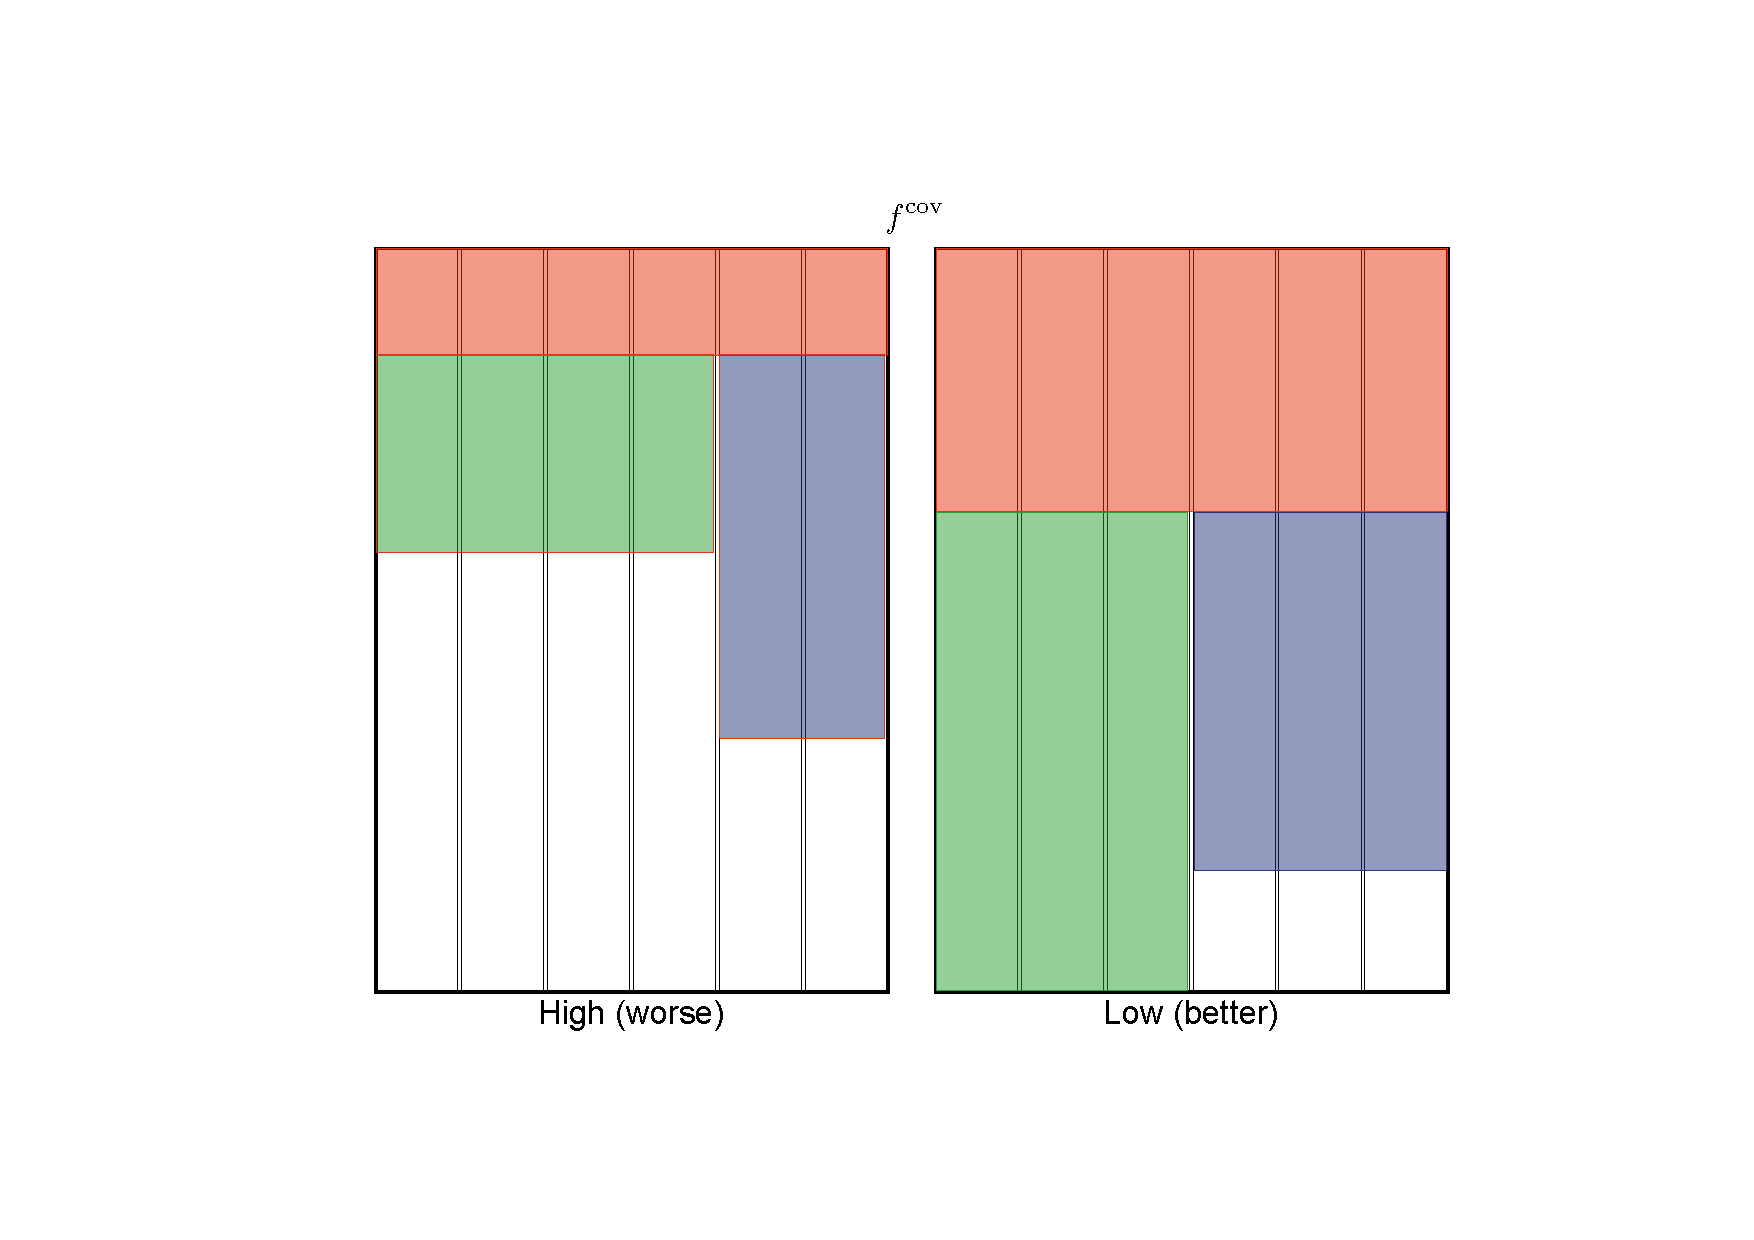
\includegraphics[width=\widthForOneImage]{img/problem-formulation/cov.pdf}
    \caption{Illustration of the Page Coverage concept: \objone\ evaluates the total unallocated white space on the page canvas, which is defined as the difference between the effective page area and the cumulative area occupied by all articles under their assigned templates and vertical elasticity levels.}
    \label{fig:page_coverage_concept}
\end{figure}

\objone\ evaluates the efficiency of the layout configuration in terms of page occupation. The mathematical goal is to minimize the total unallocated empty white space.

The total physical area occupied by an individual article \articleobj{i}\ under its assigned template \templatesel{i}\ and vertical elasticity level \elasticity{i}\ is given by $\Wtemp{\templatesel{i}} \cdot \Hscaled{i}$. The objective function accumulates the total residual empty space:

\begin{equation}
\objone = (\Weff \cdot \Heff) - \sum_{i=1}^{\numarticles} \left( \Wtemp{\templatesel{i}} \cdot \Hscaled{i} \right)
\end{equation}

By minimizing \objone, the optimization process directly drives the articles to pack tightly, maximizing layout density. Additionally, in the rare event that the single-page constraint must be relaxed due to the absolute lack of any feasible single-page configuration, \objone\ scales to represent the cumulative sum of empty white space across all utilized pages.




\subsubsection{\objthree: Text capacity integrity}

\begin{figure}[htbp]
    \centering
      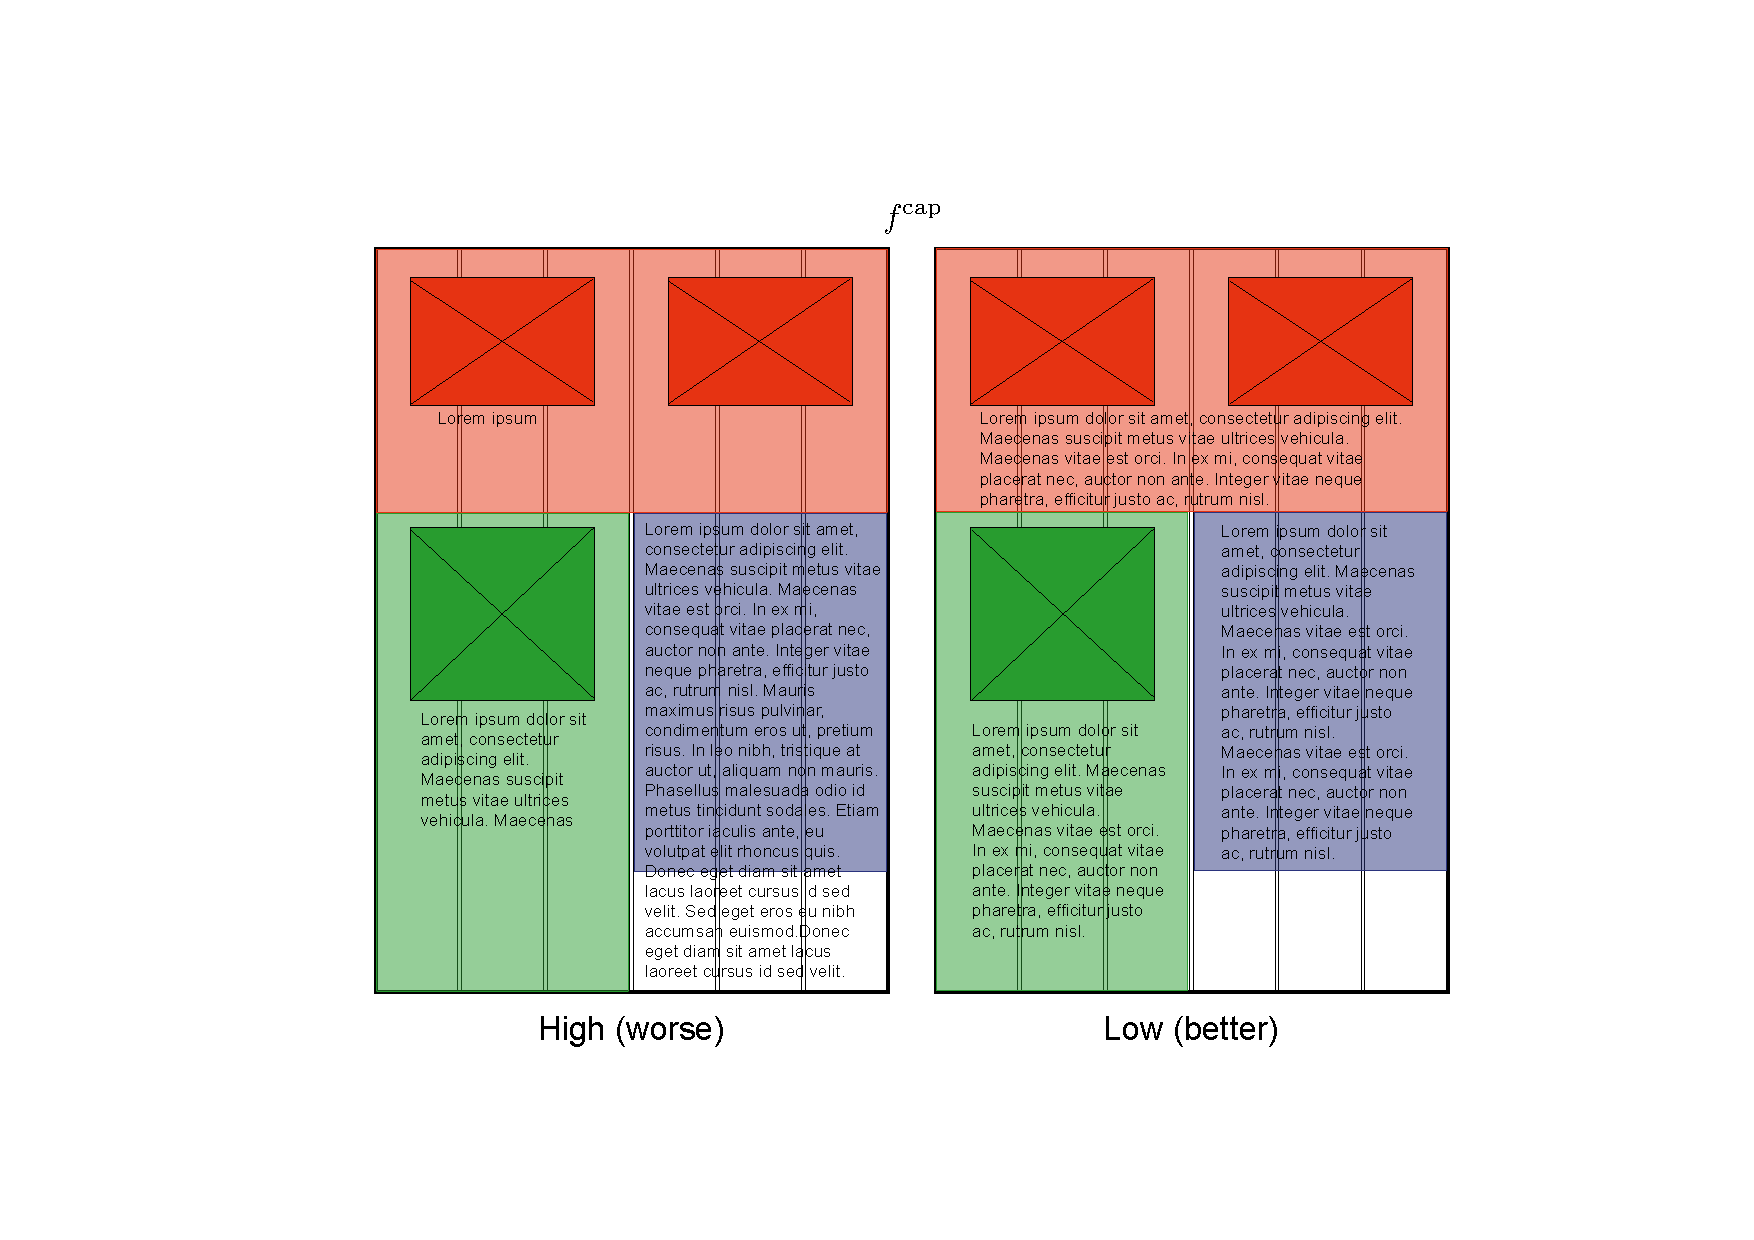
\includegraphics[width=\widthForOneImage]{img/problem-formulation/cap.pdf}

    \caption{Illustration of the Text Capacity Integrity concept: the body text of each article must fit within the capacity boundaries defined by its assigned template, which are determined by the number of active images. \objthree penalizes both under-capacity (excessive white space) and over-capacity (text clipping) scenarios.}
    \label{fig:text_capacity_integrity_concept}
\end{figure}

$\objthree$ evaluates the character count of the body text fit between the article's requirements and the text capacity boundaries of its assigned template. For each article \articleobj{i}, the character count $\Cart{i}$ must ideally fall within the permissible capacity interval $[\capacity{\templatesel{i}}[\kactive{i}, 0], \capacity{\templatesel{i}}[\kactive{i}, 1]$ dictated by the selected template $\templatesel{i}$ and the number of active images $\kactive{i} = \Nimg{i}$. 

This evaluation is modeled as a quadratic penalty function. Let $\objthreeepsilon$ be a tolerance factor that broadens the acceptable threshold bounds. The text capacity penalty $\penobjthree{i}$ for an individual article $\articleobj{i}$ is formally defined as:

\begin{subnumcases}{\penobjthree{i} =}
    0 & if $(1-\objthreeepsilon)\capacity{\templatesel{i}}[\kactive{i}, 0] \le \Cart{i} \le (1+\objthreeepsilon)\capacity{\templatesel{i}}[\kactive{i}, 1]$ \label{eq:pen_optimal} \\
    \Klower & if $\Cart{i} = 0$ and $\capacity{\templatesel{i}}[\kactive{i}, 0] > 0$ \label{eq:pen_empty} \\
    \Klower \cdot \left( \frac{\capacity{\templatesel{i}}[\kactive{i}, 0]}{\Cart{i}} - 1.0 \right)^2 & if $\Cart{i} < (1-\objthreeepsilon)\capacity{\templatesel{i}}[\kactive{i}, 0]$ and $\Cart{i} > 0$ \label{eq:pen_under} \\
    \Kupper \cdot \left( \frac{\Cart{i}}{\capacity{\templatesel{i}}[\kactive{i}, 1]} - 1.0 \right)^2 & if $\Cart{i} > (1+\objthreeepsilon)\capacity{\templatesel{i}}[\kactive{i}, 1]$ \label{eq:pen_over}
\end{subnumcases}

Where $\Klower$ and $\Kupper$ represent strictly positive penalty coefficients assigned to scale the lower and upper capacity violations, respectively.

\penobjthree{i} is designed to enforce the following principles:

\begin{itemize}
    \item Optimal fit (Eq. \ref{eq:pen_optimal}): Assigns zero penalty when the article's character count falls within the acceptable capacity limits of the template, including a small tolerance margin $\objthreeepsilon$.
    \item Empty content (Eq. \ref{eq:pen_empty}): Applies a constant penalty $\Klower$ to prevent the edge case where an article with no text is mapped to a template block that explicitly defines a text block.
    \item Under-capacity (Eq. \ref{eq:pen_under}): Imposes a quadratic penalty for text shortages (weighted by $\Klower$), preventing layouts where the assigned text container would appear excessively sparse or empty.
    \item Over-capacity (Eq. \ref{eq:pen_over}): Imposes a quadratic penalty for text overflows (weighted by $\Kupper$), strictly preventing text from being clipped or severely compressed due to a lack of spatial capacity.
\end{itemize}



The global text integrity objective function $\objthree$ aggregates the capacity deviations across all articles:
\begin{equation}
\objthree = \sum_{i=1}^{\numarticles} \penobjthree{i}
\end{equation}

By minimizing \objthree, the optimization process prioritizes solutions where text blocks are neither heavily clipped due to lack of space nor excessively sparse due to oversized containers.

\subsubsection{\objfour: Positioning of articles quality}

$\objfour$ penalizes improper positioning of articles. This objective is formulated as a linear combination of two independent penalty terms: the Heading Critical Zone penalty (\HCZ), which governs main article positioning, and the Vertical Alignment penalty (\VA), which penalizes edge misalignments between all articles:
\begin{equation}
\objfour = \HCZ + \betaweight \cdot \VA,
\end{equation}
where \betaweight\ is a strictly positive weighting parameter utilized to balance the two aesthetic criteria.

\paragraph{Privileged Critical Zone Penalty (\HCZ)} 

\begin{figure}[htbp]
    \centering
     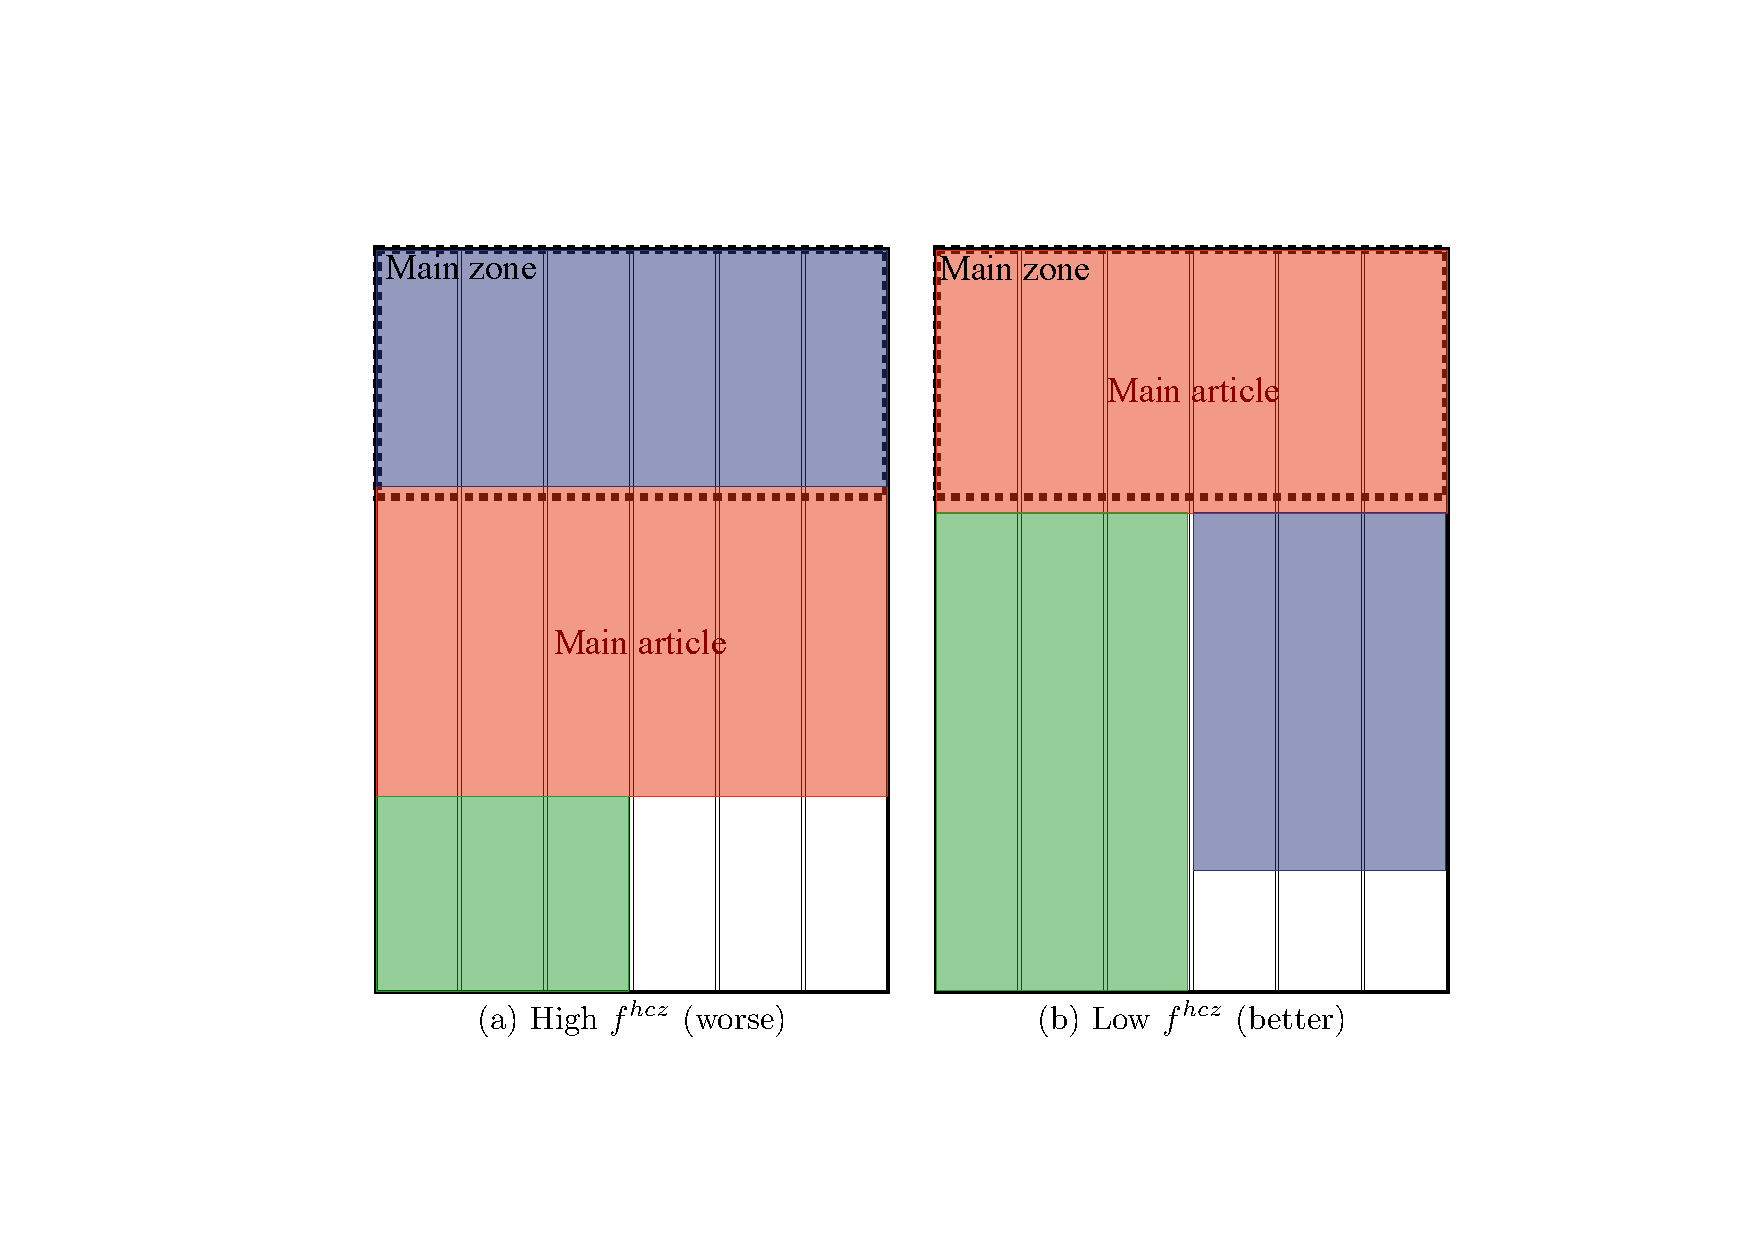
\includegraphics[width=\widthForOneImage]{img/problem-formulation/pos.pdf}
    \caption{Illustration of the Heading Critical Zone (HCZ) concept: the main article is expected to occupy a privileged upper-center region of the page canvas, defined as the first vertical third of the effective page height \Heff.}
    \label{fig:hcz_concept}
\end{figure}

To respect journalistic hierarchy, the article designated as main ($\Mainart{i} = 1$) must be positioned within a privileged geometric region of the page canvas, defined by default as the upper-center portion (the first vertical third of $\Heff$). The coordinate space of this critical zone is defined by \Zcrit:
\begin{equation}
\Zcrit = [0, \Weff] \times \left[0, \frac{1}{3}\Heff\right]
\end{equation}
The penalty evaluates the spatial coverage deficit of the main article relative to its area. Formally, the \HCZ\ penalty is defined as:
\begin{equation}
\HCZ = \sum_{i=1}^{\numarticles} \Mainart{i} \cdot \left( 1 - \frac{\Area{\bbox{i} \cap \Zcrit}}{\Area{\bbox{i}}} \right)
\end{equation}
This formulation yields a penalty of $0$ if the main article bounding box \bbox{i}\ is fully contained within \Zcrit, and approaches $1$ as the content is pushed outside the privileged zone.

\paragraph{Vertical Alignment Penalty (\VA)}

In editorial design, visual harmony heavily relies on the alignment of adjacent articles. When two horizontally neighboring articles share top or bottom boundaries that are nearly aligned, subtle offsets of a few millimeters create visual friction, making the layout appear unpolished or accidental. Conversely, when articles are substantially offset, readers perceive them as intentionally independent blocks, where strict edge continuity is no longer expected. To mathematically capture this human design principle, the Vertical Alignment penalty (\VA) evaluates horizontal sightlines by penalizing visually distracting misalignment noise.

\begin{figure}[htbp]
    \centering
     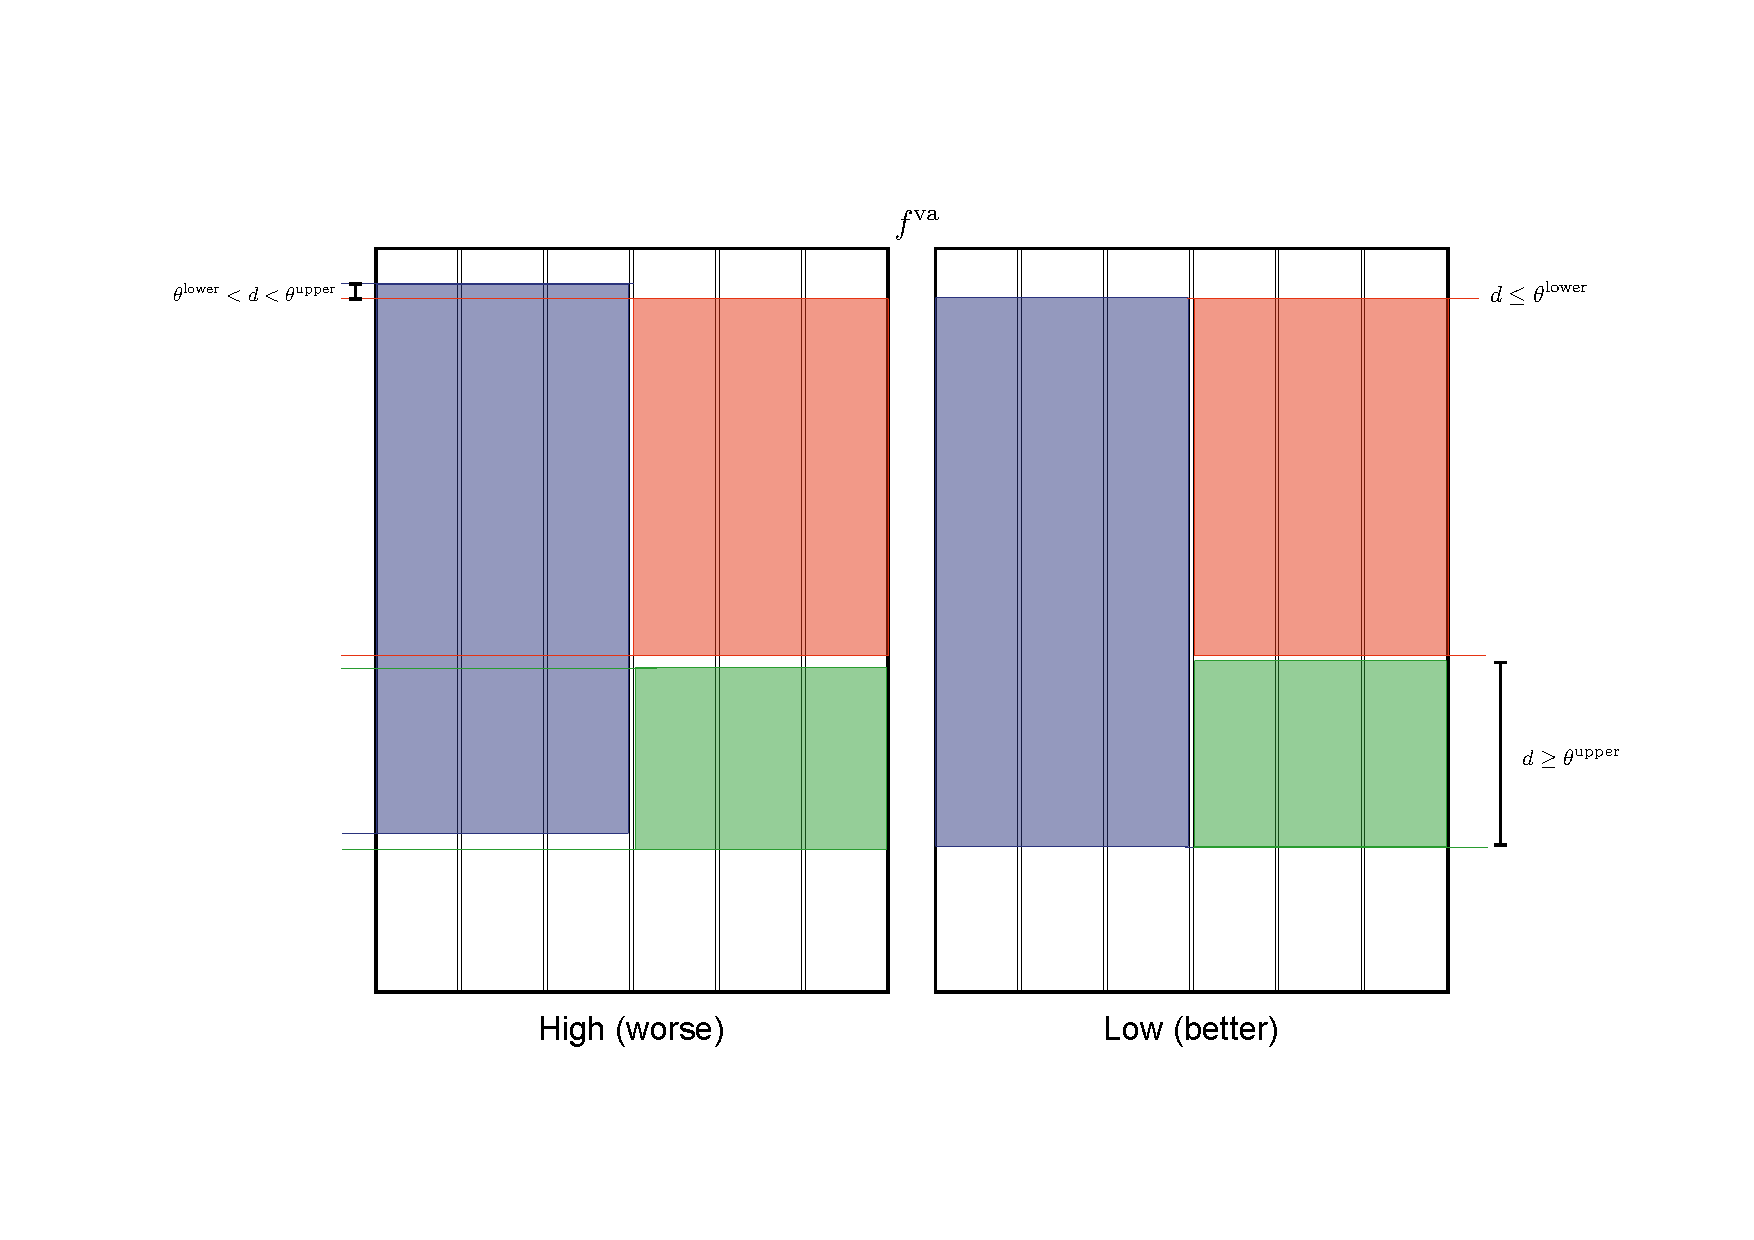
\includegraphics[width=\widthForOneImage]{img/problem-formulation/va.pdf}
    \caption{Conceptual illustration of vertical edge alignment between laterally adjacent articles: (a) optimal alignment ($d \le \threshalignlower$) forming an aligned layout, (b) misalignment noise zone ($\threshalignlower < d \le \threshalignupper$) creating visual distraction, and (c) independent separation ($d > \threshalignupper$) treated as intentionally separated articles.}
    \label{fig:vertical_alignment_concept}
\end{figure}

The alignment evaluation is restricted to pairs of articles that exhibit lateral adjacency. Formally, let $\mathcal{A}^{adj} = \{(i,j) \mid 1 \le i < j \le \numarticles \}$ be the set of unique article pairs where \articleobj{i}\ and \articleobj{j}\ share a vertical projection overlap on the page canvas. For each pair $(i,j) \in \mathcal{A}^{adj}$, let \deltaytop{i}{j}\ and \deltaybottom{i}{j}\ represent the absolute vertical distances between their top edges and bottom edges, respectively.

The alignment quality of an individual edge distance $d \in \{\deltaytop{i}{j}, \deltaybottom{i}{j}\}$ is  defined by a piecewise function relative to the effective page height \Heff:
\begin{equation}
q(d) = \begin{cases} 
1.0 & \text{if } d \le \threshalignlower, \\ 
-\frac{\alignmentScalingParameter}{\alignmentScalingParameter + d} & \text{if } \threshalignlower < d \le \threshalignupper, \\ 
0.0 & \text{if } d > \threshalignupper,
\end{cases}
\label{eq:alignment_quality}
\end{equation}
where $\alignmentScalingParameter \in \mathbb{R}^+$ is a scaling parameter that controls the steepness of the penalty curve, while $\threshalignlower$ and $\threshalignupper$ denote the lower and upper numerical thresholds for the alignment penalization zones.

The specific rationale for each operational zone in Eq. \ref{eq:alignment_quality} is established as follows:
\begin{itemize}
    \item \textbf{Optimal alignment ($d \le \threshalignlower$):} Assigns a maximum quality score of $1.0$ when edge offsets fall within an imperceptible tolerance margin, preventing artificial penalties.
    \item \textbf{Misalignment noise ($\threshalignlower < d \le \threshalignupper$):} Imposes a decaying negative quality penalty governed by $\alignmentScalingParameter$, heavily penalizing small, awkward misalignments that mimic accidental layout errors. As $d$ increases toward $\threshalignupper$, the penalty smoothly decays as the visual expectation of alignment fades.
    \item \textbf{Independent separation ($d > \threshalignupper$):} Yields a neutral score of $0.0$ for large vertical separations, treating widely separated articles as independent.
\end{itemize}

To track active misalignments across the layout, let $\mathbb{I}(d)$ be an indicator function that flags edge comparisons falling within the interaction threshold ($\threshalignupper$):
\begin{equation}
\mathbb{I}(d) = 
\begin{cases} 
1 & \text{if } d \le \threshalignupper, \\ 
0 & \text{otherwise.} 
\end{cases}
\end{equation}

The top edge quality score $\mathcal{Q}_{top}$ is computed as the normalized average over active top-edge comparisons:
\begin{equation}
\mathcal{Q}_{top} = \begin{cases} 
\frac{\sum_{(i,j) \in \mathcal{A}^{adj}} q(\deltaytop{i}{j})}{\sum_{(i,j) \in \mathcal{A}^{adj}} \mathbb{I}(\deltaytop{i}{j})} & \text{if } \sum_{(i,j) \in \mathcal{A}^{adj}} \mathbb{I}(\deltaytop{i}{j}) > 0, \\ 
1.0 & \text{otherwise.} 
\end{cases}
\end{equation}
The bottom edge quality score $\mathcal{Q}_{bottom}$ is derived identically using \deltaybottom{i}{j}. Finally, the Vertical Alignment penalty \VA\ is defined as the inversion of the equally weighted edge quality scores:
\begin{equation}
\VA = 1.0 - \left( 0.5 \cdot \mathcal{Q}_{top} + 0.5 \cdot \mathcal{Q}_{bottom} \right)
\end{equation}

Horizontal alignment evaluation is explicitly omitted from this penalty vector because horizontal grid discipline is required and enforced, as established in Equation~\ref{eq:grid_alignment}.


\subsubsection{\objtwo: Template selection editorial style}

\begin{figure}[htbp]
    \centering
     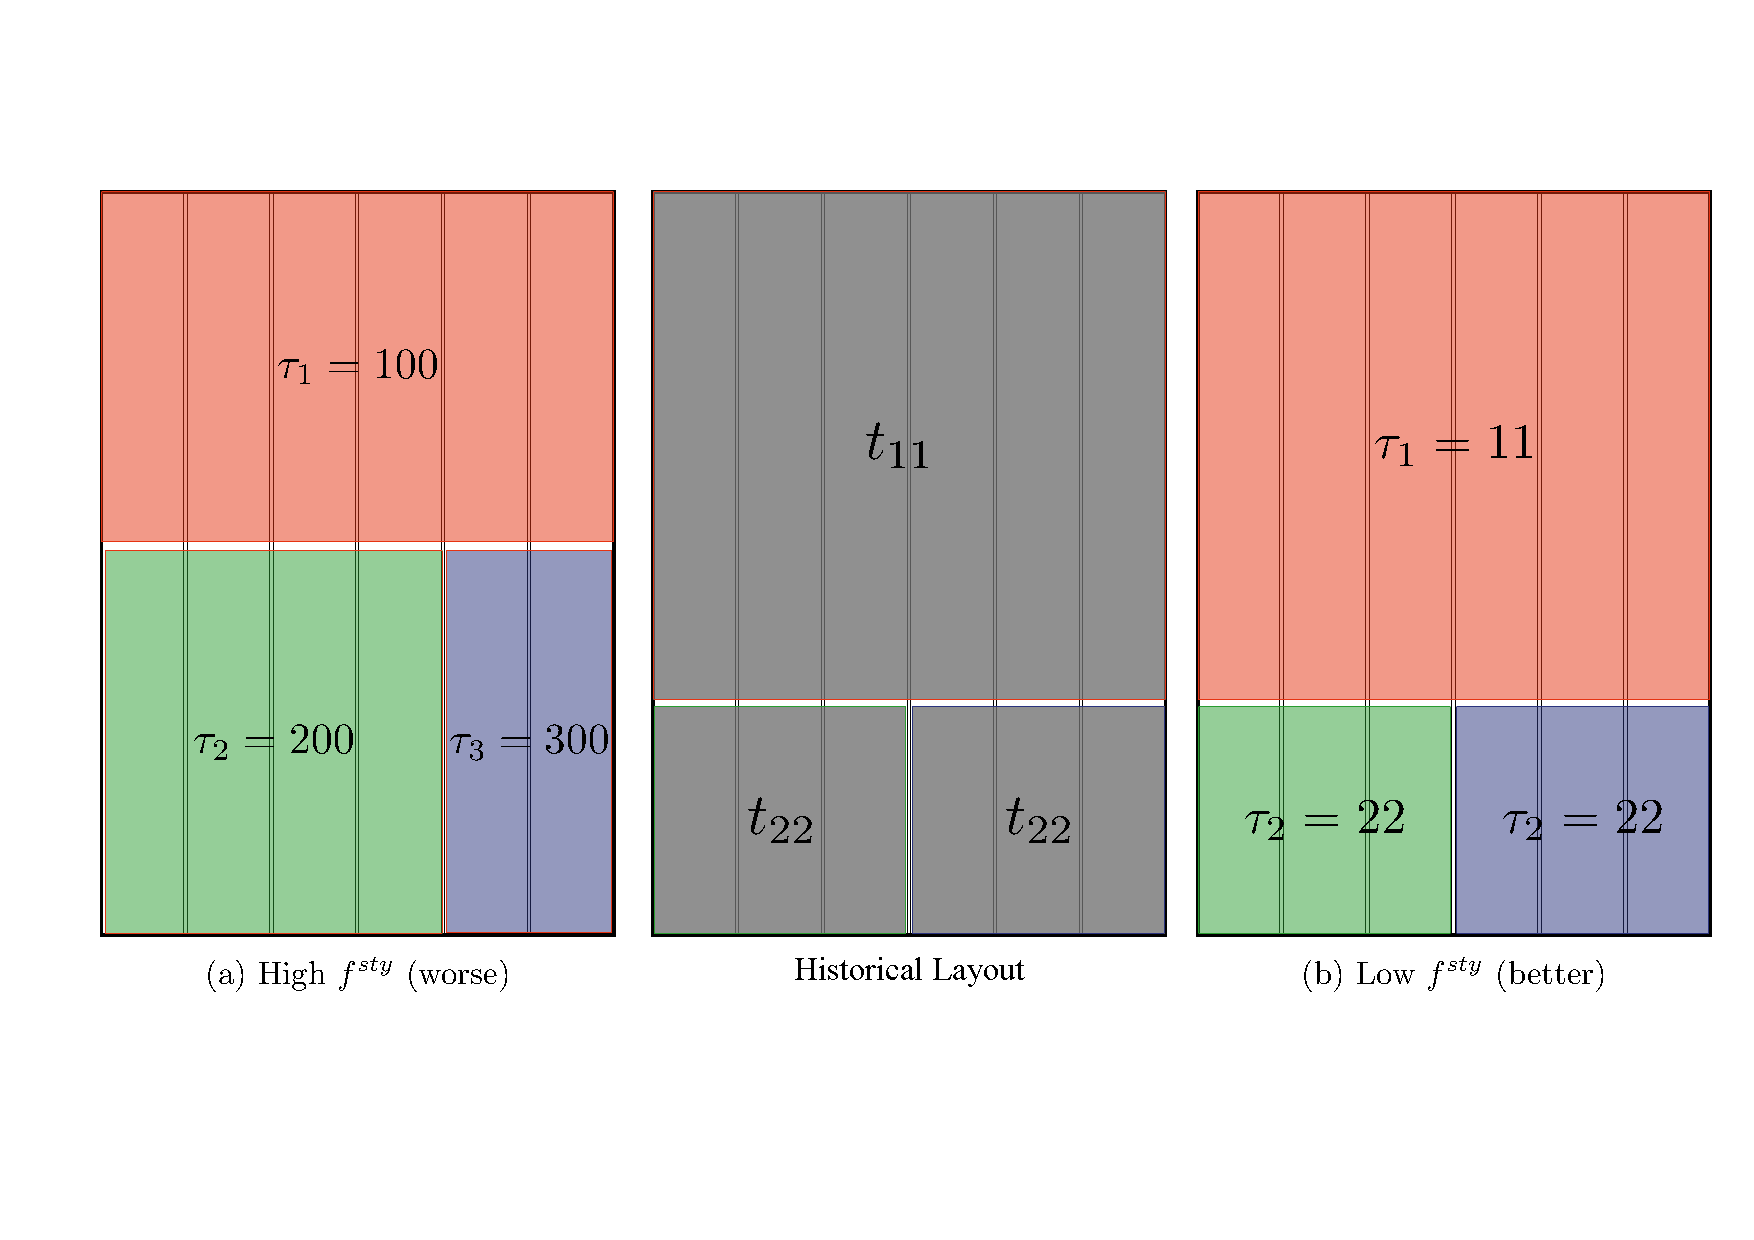
\includegraphics[width=\widthForOneImage]{img/problem-formulation/sty.pdf}
    \caption{Illustration of the Template Selection Editorial Style concept: \objtwo\ evaluates how well the assigned templates align with historical editorial template selections, capturing not only historical choices but also tacit dependencies between neighboring articles.}
    \label{fig:template_selection_editorial_style_concept}
\end{figure}

\objtwo\ evaluates the editorial quality of the layout solution $\solution$ by measuring how well the assigned templates align with historical layouts. Because newspaper layouts rely on tacit structural dependencies where the choice of a template for a given article inherently depends on its neighboring articles, this objective must be evaluated within a global page context.

Let $\Omega(\articleobj{i}, \templatesel{i} \mid \solution) \in [0, 1]$ be an abstract \textit{editorial suitability function} that quantifies the compliance of mapping article \articleobj{i}\ to template \templatesel{i}\ given the complete context of the layout solution \solution. A value of $1$ represents a perfect match according to historical editorial criteria, while a value of $0$ indicates a complete editorial mismatch. 

Since the optimization vector $\objvector{\solution}$ is formulated as a minimization problem, \objtwo\ is mathematically defined as the minimization of the aggregate editorial suitability across all arranged articles:

\begin{equation}
\objtwo = \sum_{i=1}^{\numarticles} \left( 1 - \Omega(\articleobj{i}, \templateobj{\templatesel{i}} \mid \solution) \right)
\end{equation}

By minimizing \objtwo, the optimization process drives the configuration toward layouts that preserve the signature visual identity and human design choices of templates. 

\paragraph{\objtwo\ implementation}

In particular, $\Omega(\articleobj{i}, \templateobj{\templatesel{i}} \mid \solution)$ is modeled using the \NeuralMethod (\neuralmethod) defined in Chapter~\ref{sec:gwes}. Thanks to the page-aware context deep learning architecture, \neuralmethod\ is capable of capturing the complex interdependencies between neighboring articles and their assigned templates, effectively learning the implicit editorial style, thus resolving \objtwo. Of course, this assumes that the model has been trained on a sufficiently large and representative historical dataset of newspaper layouts, in the exact same way as described in Chapter~\ref{sec:gwes}. Given this, $\Omega(\articleobj{i}, \templateobj{\templatesel{i}} \mid \solution)$ is formally defined as:

\begin{equation}
\Omega(\articleobj{i}, \templateobj{\templatesel{i}} \mid \solution) = \neuralmethod(\articleobj{i}, \templateobj{\templatesel{i}} \mid \solution),
\end{equation}

where \neuralmethod\ is considered as a pre-trained model that outputs a normalized suitability score in the range $[0, 1]$ for each article-template pair within the context of the complete solution \solution.
